\documentclass[12pt]{report}

\usepackage[T1]{fontenc}
\usepackage[utf8]{inputenc}

% Math
\usepackage{amsmath}
\usepackage{amsfonts}
\usepackage{amssymb}
\usepackage{amsthm}

% Algorithm & code listing
\usepackage{algorithm}
\usepackage{algpseudocode}
\usepackage{titling}
\usepackage{listings}
\usepackage{enumitem}

% Graphics & figures
\usepackage{graphicx}
\usepackage[pdf]{graphviz}
\usepackage{tikz}
\usetikzlibrary{automata,arrows,positioning,calc}

% Bibliotheq
\usepackage{biblatex}
\addbibresource{thesis.bib}

% MACROS
\newcommand*{\QED}{\hfill\ensuremath{\square}}
\newcommand{\stirlingii}{\genfrac{\{}{\}}{0pt}{}}

\theoremstyle{definition}
\newtheorem{definition}{Definition}[section]

\newtheorem{theorem}{Theorem}
\newtheorem{lemma}[theorem]{Lemma}

\newcommand{\subtitle}[1]{%
  \posttitle{%
    \par\end{center}
  \begin{center}\large#1\end{center}
  \vskip0.5em}%
}

\begin{document}

%%%%%%%%%%%%%%%%%%%%%%%% Title Page %%%%%%%%%%%%%%%%%%%%%%%%
\begin{titlepage}
  \begin{center}
    {\LARGE \textbf{Bayesian Parameter Synthesis of Markov Population Models}}
    \\[1cm]
    {\Large \textbf{Master Thesis}}
    \\[1cm]
    {\Large Submitted by}
    \\[0.5cm]
    {\LARGE \textbf{Nhat-Huy Phung}}
    \\[0.5cm]
    {\Large at the}
    \\[0.5cm]
    
\includegraphics[width=0.5\textwidth]{figures/unisignet-klein.jpg}
    \\[1cm]
    {\large \textbf{Modeling of Complex, Self-organising Systems}}
    \\[1cm]
    {\large \textbf{Department of Computer and Information Science}}
    \\[2cm]
    \begin{minipage}[c]{\textwidth}
      \begin{description}[style=multiline]
        \item {\large \textbf{1. Supervised by:} Prof. Dr. Tatjana Petrov }
        \item {\large \textbf{2. Supervised by:} Prof. Dr. Stefan Leue }
      \end{description}
    \end{minipage}
    \vfill
    {\LARGE \textbf{Konstanz, 2021}}
  \end{center}
\end{titlepage}
\tableofcontents

\chapter*{Acknowledgements}
\thispagestyle{empty}

First and foremost, I would like to express its gratitude and appreciation to my supervisor
Prof.Dr. Tatjana Petrov. Without her motivation, advice, supports, and feedback on my implementation
and writing, this thesis would be far from being done.\\

\noindent Working in the research group MCSS (modeling of complex, self-organising systems) is an excellent
experience. I would like to thank the members of MCSS group, Matej Hajnal, Stefano Tognazzi, and
Denis Repin for their nice discussions and feedback on the technical and theoretical aspects of my
work.\\

\noindent My deep gratitude goes to my family. Despite of being thousands of kilometers away, they are
always the best source of support and encouragement. A special thank is for Lu Dinh, for her
endless love and encouragement.\\

\clearpage

\begin{abstract}
    Population models are mathematical models to study the dynamics of a population. Markov
    population processes are Markov chains of continuous or discrete time, in which a state tracks
    population size of each of the involved species. We study a framework for data-informed
    parameter synthesis of parametric Markov population processes. Given experimental data for the
    population at its steady-state, parameter synthesis aims to find a set of parameters satisfying
    a temporal property of interest. We assume that experimental observations of the population are
    available at steady-state. We design and compare performance of a Bayesian framework for
    parameter synthesis in two cases: (i) when the exact likelihood function of the property of
    interest is computed in a pre-processing step, and (ii) when it has to be approximated by means
    of Monte-Carlo methods (it is likelihood-free). The frameworks are constructed with different
    sampling and optimization techniques to approximate the posterior distribution. We evaluate the
    frameworks using various population models of different sizes, using synthetic data generated
    from a known true parameter. By measuring the distance between estimated parameters and true
    parameters, and by visualize synthesized parameter values with their corresponding posterior
    estimate, we show that both frameworks can derive a set of satisfying parameter values and an
    estimation that is close to the true parameter. Furthermore, results show that the
    likelihood-free framework is overall performing better.
\end{abstract}


\chapter{Introduction}
\section{Motivation}
Firstly introduced by Kingsman \cite{kingman1969markov}, Markov population models  are finite
state-space, stochastic models widely used in modeling complex and dynamical systems. In a Markov
population model, each state represents the number of individuals, and the transitions among states
represent the increase or decrease of a population. In general, Markov population models study the
population dynamics of a system of interest. For example, Markov population processes are able to
model:
\begin{itemize}
      \item Number of online nodes in a distributed system.
      \item Number of surviving individuals in an epidemic model.
\end{itemize}
Studying the Markov population model has challenges. First, model state space exponentially expands
as we capture more attributes and behavior of the system of interest. The explosion of state-space
makes model checking of the Markov population model computationally intensive. Second, in a Markov
population model, such as Discrete-time Markov Chain, initial and transition probabilities are known
a priori. To encompass unknown attributes of a system, we introduce parametric Markov population
models. In a parametric Markov population model, each transition is a rational function of
parameters. As parameters represent unknown features of the system, it gives the following research
questions
\begin{itemize}
      \item Given a set of data collected by observing the system, what can we know about its
            parameters?
      \item Which values of parameters instantiate a model that satisfies a specific property of
            interest?
\end{itemize}
Parameter synthesis is an emerging research direction on probabilistic model checking. Katoen
\cite{katoen2016probabilistic} defines the parameter synthesis problem for the parametric
discrete-time Markov chain to find a set of parameter values that satisfy a given reachability
property. In this thesis, we combine Bayesian parameter inference and parameter synthesis. The
result parameters (i) satisfy the property of interest, and (ii) are likely to produce given
steady-state data. Contributions of the thesis are
\begin{itemize}
      \item We are presenting and implementing a data-informed, Bayesian framework on parameter
            synthesis of parametric Discrete-time Markov chain. The frameworks work in two cases:
            (i) when the exact likelihood function of the property of interest is available, and
            (ii) when it has to be approximated utilizing Monte-Carlo methods.
      \item We compare the performances of optimization methods used to approximate posterior
            distribution on various case studies.
      \item We evaluate the scalability of the frameworks with different sizes of model state-space.
\end{itemize}

\section{Related works}
%% Frameworks from molyneux
The frameworks presented in this thesis are based on ABC-SMC framework \cite{molyneux2019bayesian}
and ABC-(SMC)2 \cite{molyneux2020abc} by Molyneux et al. However, the ABC-SMC and ABC-(SMC)2
frameworks synthesize parameters for CTMC and check the CTMC model agains CSL property. In
parametric DTMC, since the symbolic rational function of PCTL property is obtainable
\cite{daws2004symbolic}, we based on Del Moral \cite{del2006sequential} and Daviet
\cite{daviet2018inference} to construct an algorithm based on evaluation of symbolic rational
function, then benchmark it againts the approach based on only simulation.

%% Model checking
The theoretical background of model checking discrete-time Markov chain is presented by Baier et al.
\cite{baier2008principles}. Katoen \cite{katoen2016probabilistic} presents a tutorial to model check
parametric discrete-time Markov chain and current methods on parameter synthesis . More in-depth
surveys and discoveries on parametric model checking and parameter synthesis is presented by Junges
\cite{junges2020parameter} and Hutschenreiter \cite{hutschenreiter2017parametric}.

%% Bayesian inference: optimzation methods
Markov Chain Monte Carlo sampling algorithms used in this thesis are presented by Metropolis
\cite{metropolis1953equation}, and Hastings \cite{hastings1970monte}. Del Moral
\cite{del2006sequential} designed Sequential Monte Carlo to address the problem of Markov Chain
Monte Carlo. A comparision between different Monte Carlo sampling algorithms, including Markov-chain
Monte Carlo and Sequential Monte Carlo is presented in \cite{daviet2018inference}. Silk
\cite{silk2012optimizing} and Filippi \cite{filippi2013optimality} discussed different approaches on
the perturbation kernel selection of Sequential Monte Carlo and Sequential Monte Carlo with
Approximate Bayesian Computation algorithms.

%% Tools: PRISM and STORM
The model checking step in the frameworks presented by this thesis are implemented using Storm model
checker \cite{hensel2020probabilistic}. Storm provides well documented and easy to use APIs to embed
model checking to software projects programmatically. However, Storm does not support Statistical
Model Checking. Thus, the Statistical Model Checking step in simulation-based frameworks is
implemented using PRISM \cite{kwiatkowska2011prism}.

\section{Structure of the thesis}
The content in this thesis is organized to 7 chapters:
\begin{itemize}
      \item \textbf{Chapter 1} introduces motivations and goals of this research.
      \item \textbf{Chapter 2} presents the theoretical background on probabilistic model checking,
            include discrete stochastic models and their  corresponding temporal logics.
      \item \textbf{Chapter 3} presents essential concepts on Bayesian inference, including sampling
            and optimization algorithms.
      \item \textbf{Chapter 4} reviews the state-of-the-art works of other researchers on the
            problem of parameter synthesis.
      \item \textbf{Chapter 5} present Bayesian parameter synthesis frameworks.
      \item \textbf{Chapter 6} describes case studies and benchmarks presented frameworks under
            different setups.
      \item \textbf{Chapter 7} conclusion and possible future works.
\end{itemize}


\chapter{Preliminaries}
 {\color{red}
  \begin{itemize}
      \item probabilistic model checking
      \item parameter synthesis landscape
      \item bayesian inference of parameter
  \end{itemize}
 }

\section{Probabilistic model checking}
\subsection{Discrete-time probabilistic models}
%% DEFINE Discrete time probabilistic models
\begin{definition}[Discrete Time Markov Chain]
    A Discrete Time Markov Chain (DTMC) is a tuple $(S,\mathbf{P}, S_{init}, AP,
        L)$ \cite{baier2008principles}
    \begin{itemize}
        \item $S$ is a countable non-emty set of \textit{states}
        \item $\mathbf{P}:S\times S \rightarrow [0,1]$ is the \textit{transition probability}
              function, s.t $$\sum_{s'\in S}\mathbf{P}(s, s') = 1$$
        \item $S_{init}: S \rightarrow [0,1]$ is the \textit{initial distribution},
              s.t  $$\sum_{s'\in S}S_{init}(s') = 1$$
        \item $AP$ is a set of \textit{atomic propositions}
        \item $L: S \rightarrow 2^{AP}$ is the labelling function on states.
    \end{itemize}
\end{definition}

%% DEFINE Probabilistic model checking of LTL and CTL properties
\subsection{Temporal properties on probabilistic models}
%% DEFINE CTL property
Over CTL properties, we define the set of PCTL properties, in which we ask the probability to have a CTL property satisfied.
%% DEFINE PCTL property
\begin{definition}[PCTL syntax] The syntax of PCTL is defined as follow
    \begin{align*}
        \Phi & ::== \text{true} \;|\; a \;|\; \Phi \;|\; \Phi \wedge \Phi \;|\; \Phi \vee \Phi \;|\;  P_{\sim  p}[\phi] \\
        \phi & ::== X\Phi \;|\; \Phi U \Phi
    \end{align*}
\end{definition}

\subsection{Parametric model and parameter synthesis}


\section{Bayesian Inference}
\subsection{Bayes' theorem}
\subsection{Posterior conjugation}
\subsection{Metropolis-Hastings algorithm}
\subsection{Selection of prior distribution}
The selection of prior distribution has strong effect on the result [what result
        specifically?] of a Bayesian inference {\color{red}[Citation needed]}.

\section{Bayesian verification}
\chapter{Related works}

%% Probabilistic model checking and parameter synthesis
The current research progress on probabilistic model checking is studied thoroughly by Katoen and Baier et al \cite{baier2008principles}. Katoen et al. \cite{katoen2016probabilistic} briefly summarized important aspect of probabilistic model checking.

%% Bayesian verification
Polgreen et al \cite{polgreen2016data} presents a method for bayesian inference of pMC parameters in

%% Tools: PRISM and STORM

The definition and model checking of DTMC and pMC is studied by
\cite{baier2008principles}, \cite{hutschenreiter2017parametric}, and \cite{katoen2016probabilistic}.\\
Bayesian inference of pMC parameters is studied in \cite{polgreen2016data} and
\cite{jha2009bayesian}. In \cite{polgreen2016data}, the authors developed
methods to synthesize parameters to satisfy a given set of PCTL properties. In
\cite{jha2009bayesian}, the authors presented methods to perform model checking
of biological system using Bayesian statistic. The authors in
\cite{jha2009bayesian} uses a Bayesian hypothesis test, where $H_0$ is the null
hypothesis that the model satisfies a PCTL $P$, and alternative hypothesis $H_1$
is that the system does not satisfies $P$. Similar approach to the parameter
estimation in this project is described by \cite{hussain2015automated}.\\
In this project, we use bee colony model semantics from \cite{hajnal2019data}.
The methods and implementation in this project is designed to extend the results
of \cite{hajnal2019data} and its tool \textit{DiPS}

storm drawback: it does not support discrete event simulation

In \cite{molyneux2020abc} the author introduces the same approach but it is to use on CSL properties and CTMC.
\chapter{Bayesian frameworks for parameter synthesis.}

\section{Bayesian frameworks with rational functions}
\newpage
As we have analytical form for both target property and likelihood function, we can propose a Markov
chain Monte-Carlo algorithm. In this case we use Metropolis-Hastings algorithm, with rational
function evaluation and model checking is performed before the calculation of acceptance rate.
\begin{algorithm}[H]
    \caption{Markov chain Monte-Carlo with rational functions}
    \label{rf-mcmc-alg}
    \hspace*{\algorithmicindent} \textbf{Input:}
    \begin{itemize}
        \item $\mathcal{M}_\theta$: parametric Discrete-Time Markov chain of parameter $\theta$
        \item $\Phi$: bounded reachability property of interest.
        \item $RF_\Phi(\theta)$: rational function of target property.
        \item $\pi(\theta)$: prior distribution on $\theta$.
        \item $N_{MH}$: length of particle trace.
        \item $Q(\theta^t|\theta^{t-1})$: transition kernel.
        \item $D_{obs}$: observed data.
        \item $P(D_{obs}|\theta):$ likelihood function.
    \end{itemize}
    \hspace*{\algorithmicindent} \textbf{Output:}
    \begin{itemize}
        \item $(\theta_1,\ldots,\theta_{N_{MH}})$: $N_{MH}$ sampled particles.
        \item $(w_1,\ldots,w_{N_{MH}})$: corresponding weights of sampled particles.
    \end{itemize}
    \begin{algorithmic}[1]
        \Procedure{RF-MCMC}{}
        \State $sat \leftarrow False$
        \While{$sat = False$}
            \State Draw $\theta_{cand}$ from $\pi(\theta)$
            \State Evaluate $val \leftarrow RF_{\Phi}(\theta)$
            \If{$val$ satisfies the boundary of $\Phi$}
                \State $sat \leftarrow True$
            \EndIf
        \EndWhile
        \State $\theta_1 \leftarrow  \theta_{cand}$
        \State $w_1 \leftarrow  \ln(P(D_{obs}|\theta_{cand}))$
        \algstore{algctx}
\end{algorithmic}
\end{algorithm}

\begin{algorithm}                     
\begin{algorithmic}[H]
\algrestore{algctx}
        \State $i \leftarrow 2$
        \While{$i \leq N_{MH}$}
            \State $sat \leftarrow False $
            \While{$sat = False$}
                \State Draw $\theta_{cand}$ from $Q(\theta'|\theta_{i-1})$
                \State Evaluate $val \leftarrow RF_{\Phi}(\theta)$
                \If{$val$ satisfies the boundary of $\Phi$}
                    \State $sat \leftarrow True$
                \EndIf
            \EndWhile
            \If{ $\ln(P(D_{obs}|\theta_{cand})) - \ln(P(D_{obs}|\theta_{i-1})) > 0$ }
                \State $\theta_i \leftarrow \theta_{cand}$
                \State $w_i \leftarrow \ln(P(D_{obs}|\theta_{cand}))$
                \State $i \leftarrow i + 1$
            \Else
                \State Draw a random number $u$ from $Uniform(0,1)$
                \If{$u \leq \xi$, ($\xi$ small, e.g $10^{-2}$)}
                    \State $\theta_i \leftarrow \theta_{cand}$
                    \State $w_i \leftarrow \ln(P(D_{obs}|\theta_{cand}))$
                    \State $i \leftarrow i + 1$
                \EndIf
            \EndIf
        \EndWhile
        \State Return $(\theta_1,\ldots,\theta_{N_{MH}})$, $(w_1,\ldots,w_{N_{MH}})$
        \EndProcedure
    \end{algorithmic}
\end{algorithm}

We can also use Sequential Monte-Carlo sampling method.

\begin{algorithm}[H]
    \caption{Sequential Monte-Carlo with rational functions}
    \label{rf-smc-alg}
    \hspace*{\algorithmicindent} \textbf{Input:}
    \begin{itemize}
        \item $\mathcal{M}_\theta$: parametric Discrete-Time Markov chain of parameter $\theta$
        \item $\Phi$: bounded reachability property of interest.
        \item $RF_\Phi(\theta)$: rational function of target property.
        \item $\pi(\theta)$: prior distribution on $\theta$.
        \item $N$: number of particles in the Sequential Monte-Carlo trace.
        \item $M$: number of pertubation kernels
        \item $F_t(\theta^t | \theta^{t-1}_1,\ldots,\theta^{t-1}_N), 1\leq t \leq M$: pertubation kernels
        \item $N_{MH}$: number of particles in each Metropolis-Hastings step.
        \item $Q_t(\theta^t|\theta^{t-1}), 1 \leq t \leq N_{MH}$: transition kernel for Metropolis-Hastings step.
        \item $D_{obs}$: observed data for Bayesian inference or its summary statistic $S_{obs}$
        \item $P(D_{obs}|\theta):$ likelihood function.
    \end{itemize}
    \hspace*{\algorithmicindent} \textbf{Output:}
    \begin{itemize}
        \item $(\theta_1,\ldots,\theta_N)$: $N$ sampled particles.
        \item $(w_1,\ldots,w_N)$: corresponding weights of sampled particles.
    \end{itemize}
    \begin{algorithmic}[1]
        \Procedure{RF-SMC}{}
        \State $i \leftarrow 1$
        \While{$i \leq N$} \algorithmiccomment {SMC initialization}
            \State Draw $\theta$ from $\pi(\theta)$
            \State $\theta_i \leftarrow \theta$
            \State $w_i \leftarrow P(D_{obs}|\theta_i)$
        \EndWhile
    \algstore{algctx}
\end{algorithmic}
\end{algorithm}

\begin{algorithm}                     
\begin{algorithmic}[H]
    \algrestore{algctx}
        \State $t \leftarrow 1$
        \While{$t \leq M$}
            \State $i \leftarrow 1$ \algorithmiccomment{SMC correction step}
            \While{$i \leq N$}
                \State $w'_i \leftarrow \frac{w_i}{\sum_{i=1}^N w_i} $
            \EndWhile
            \State Sample with replacement $(\theta'_1,\ldots,\theta'_N)$ \algorithmiccomment{SMC selection step} \\\hspace{1.5cm} from $(\theta_1,\ldots,\theta_N)$ with probabilities $(w'_1,\ldots,w'_N)$ 
            \State $(\theta_1,\ldots,\theta_N) \leftarrow (\theta'_1,\ldots,\theta'_N)$ 
            \State $i \leftarrow 1$
            \While{$i \leq N$} \algorithmiccomment {SMC pertubation step}
                \State Draw $\hat{\theta}^t_i$ from $F_t(\theta^t | \theta^{t-1}_1,\ldots,\theta^{t-1}_N), 1\leq t \leq M$
                \State $(\theta^*_1,\ldots,\theta^*_{N_{MH}}), (w^*_1,\ldots,w^*_{N_{MH}}) \leftarrow RF-MCMC(\hat{\theta}^t_i)$
                \State $\theta_i \leftarrow \theta^*_{N_{MH}}$
                \State $w_i \leftarrow w^*_{N_{MH}}$
            \EndWhile
        \EndWhile
        \State Return $(\theta_1,\ldots,\theta_{N})$, $(w_1,\ldots,w_{N})$
        \EndProcedure
    \end{algorithmic}
\end{algorithm}

\section{Bayesian frameworks without rational functions}

Without the availability of analytical form of observational and interested properties, we face the
following obstacles:
\begin{itemize}
    \item \textbf{Absence of likelihood functions:} As the rational functions for properties are not
    available, we do not have the analytical form of likelihood. The abscence of likelihood suggests
    to exploit \textit{likelihood-free methods}. In this framework we use \textit{Approximate
    Bayesian Computation} in combination with \textit{Sequential Monte-Carlo method}.
    \item \textbf{Absence of rational function for verification of bounded path property:} the
    satisfaction of an instantiated model to a bounded path property cannot be computed. In the case
    that the number of states is too large, we use \textit{Statistical Model Checking}.
\end{itemize}
For this case we present Statistical Model Checking, Approximate Bayesian Computation - Sequential
Monte-Carlo method \textit{SMC-ABC-SMC} framework.

\begin{algorithm}[H]
    \caption{Sequential Monte-Carlo with Approximate Bayesian Computation and Statiscal Model Checking}
    \label{smc-abc-smc-alg}
    \hspace*{\algorithmicindent} \textbf{Input:}
    \begin{itemize}
        \item $\mathcal{M}_\theta$: parametric Discrete-Time Markov chain of parameter $\theta$
        \item $\Phi$: bounded reachability property of interest.
        \item $RF_\Phi(\theta)$: rational function of target property.
        \item $\pi(\theta)$: prior distribution on $\theta$.
        \item $N$: number of particles in the Sequential Monte-Carlo trace.
        \item $M$: number of pertubation kernels
        \item $F_t(\theta^t | \theta^{t-1}_1,\ldots,\theta^{t-1}_N), 1\leq t \leq M$: pertubation kernels
        \item $N_{MH}$: number of particles in each Metropolis-Hastings step.
        \item $Q_t(\theta^t|\theta^{t-1}), 1 \leq t \leq N_{MH}$: transition kernel for Metropolis-Hastings step.
        \item $D_{obs}$: observed data for Bayesian inference or its summary statistic $S_{obs}$
        \item $P(D_{obs}|\theta):$ likelihood function.
    \end{itemize}
    \hspace*{\algorithmicindent} \textbf{Output:}
    \begin{itemize}
        \item $(\theta_1,\ldots,\theta_N)$: $N$ sampled particles.
        \item $(w_1,\ldots,w_N)$: corresponding weights of sampled particles.
    \end{itemize}
    \begin{algorithmic}[1]
        \Procedure{SMC-ABC-SMC}{}
        \State $i \leftarrow 1$
        \While{$i \leq N$} \algorithmiccomment {SMC initialization}
            \State Draw $\theta$ from $\pi(\theta)$
            \State $\theta_i \leftarrow \theta$
            \State $w_i \leftarrow P(D_{obs}|\theta_i)$
        \EndWhile
    \algstore{algctx}
\end{algorithmic}
\end{algorithm}

\begin{algorithm}                     
\begin{algorithmic}[H]
    \algrestore{algctx}
        \State $t \leftarrow 1$
        \While{$t \leq M$}
            \State $i \leftarrow 1$ \algorithmiccomment{SMC correction step}
            \While{$i \leq N$}
                \State $w'_i \leftarrow \frac{w_i}{\sum_{i=1}^N w_i} $
            \EndWhile
            \State Sample with replacement $(\theta'_1,\ldots,\theta'_N)$ \algorithmiccomment{SMC selection step} \\\hspace{1.5cm} from $(\theta_1,\ldots,\theta_N)$ with probabilities $(w'_1,\ldots,w'_N)$ 
            \State $(\theta_1,\ldots,\theta_N) \leftarrow (\theta'_1,\ldots,\theta'_N)$ 
            \State $i \leftarrow 1$
            \While{$i \leq N$} \algorithmiccomment {SMC pertubation step}
                \State Draw $\hat{\theta}^t_i$ from $F_t(\theta^t | \theta^{t-1}_1,\ldots,\theta^{t-1}_N), 1\leq t \leq M$
                \State $(\theta^*_1,\ldots,\theta^*_{N_{MH}}), (w^*_1,\ldots,w^*_{N_{MH}}) \leftarrow RF-MCMC(\hat{\theta}^t_i)$
                \State $\theta_i \leftarrow \theta^*_{N_{MH}}$
                \State $w_i \leftarrow w^*_{N_{MH}}$
            \EndWhile
        \EndWhile
        \State Return $(\theta_1,\ldots,\theta_{N})$, $(w_1,\ldots,w_{N})$
        \EndProcedure
    \end{algorithmic}
\end{algorithm}

\section{Selection of pertubation kernel}
Selection of pertubation kernel is mentioned in \cite{filippi2013optimality}. In this thesis, we use
component-wise uniform kernel:

\chapter{Case study}
\section{Zeroconf}
\subsection{System}
\subsection{Data}
\subsection{Model}
\subsection{Properties}
\subsection{Evaluation}

\section{Bees colony}
\subsection{System}
We study the collective behavior of a bee colony. Each bee in a colony
possibly stings after observing a threat in the surrounding environment, and
warn other bees by releasing a special substance, pheromone. By sensing the
pheromone released in the environment, other bees in the colony may also
sting. However, since stinging leads to the termination of an individual bee,
it reduces the total defense capability as well. With parametric Discrete-time
Markov chain as the model, we study how the actions of a single bee change
with regarding to the colony size of and pheromone amount. 

\subsection{Model}
Assume that each bee in a colony decides its next action (to sting or not to
sting) based only on the current state of the environment, and the number of
bees who sting or not sting can be modeled as a Markov process. To reduce the
complexity of the model, we make another assumption that the states of the bees
colony are observed after uniform time duration, hence the model is of
discrete-time.There are 3 assumptions on the system:
\begin{enumerate}
    \item Each bee release an unit amount of pheromone immediately after stinging.
    \item A bee dies after stinging and releasing pheromone. In the other words, no
          bee can sting more than once.
    \item Stinging behaviour only depends on the concentration of pheromone in the
          environment.
\end{enumerate}
Under these assumption, a bee colony can be viewed as a set of agents (bees)
interact with each other in a closed environment with the appearance of a factor
\textit{pheromone}. Afterward, the agent has probability to commit an action, namely \textit{sting}.
The agent is eliminated from environment after stinging.
Assume that we have a colony of $n$ bees initially. As aforementioned, an individual bee
is terminated after it stings. Thus, at the end of experiment, the number of
bees is $n'\in\{0,1,\ldots,n\}$. We model the bee colony with a DTMC
$\mathcal{M}=(S,\mathbf{P}, S_{init}, AP,L)$, such that
\begin{itemize}
    \item $|S_{init}|=1$
    \item There exists $n+1$ tSCCs which encode the population at the end of the experiment.
\end{itemize}
Semantics of Markov population models for bees colony are developed by
\cite{hajnal2019data}.
\subsection{Properties}
\subsection{Evaluation}


\section{SIR model}
\subsection{System}
\textit{SIR} model  is a population model, which is widely used in modeling epidemics. In a \text{SIR} model, each individual is of one among three types:
\begin{itemize}
    \item \textit{Susceptible (S)}
    \item \textit{Infected (S)}
    \item \textit{Recovered (S)}
\end{itemize}
\begin{align*}
    S + I \xrightarrow{\alpha} 2I \\
    I \xrightarrow{\beta} R
\end{align*}

\subsection{Data}
\subsection{Model}
Example of an SIR CTMC model with initial population $(S_0, I_0, R_0) = (3,1,0)$
\begin{figure}
    \centering
    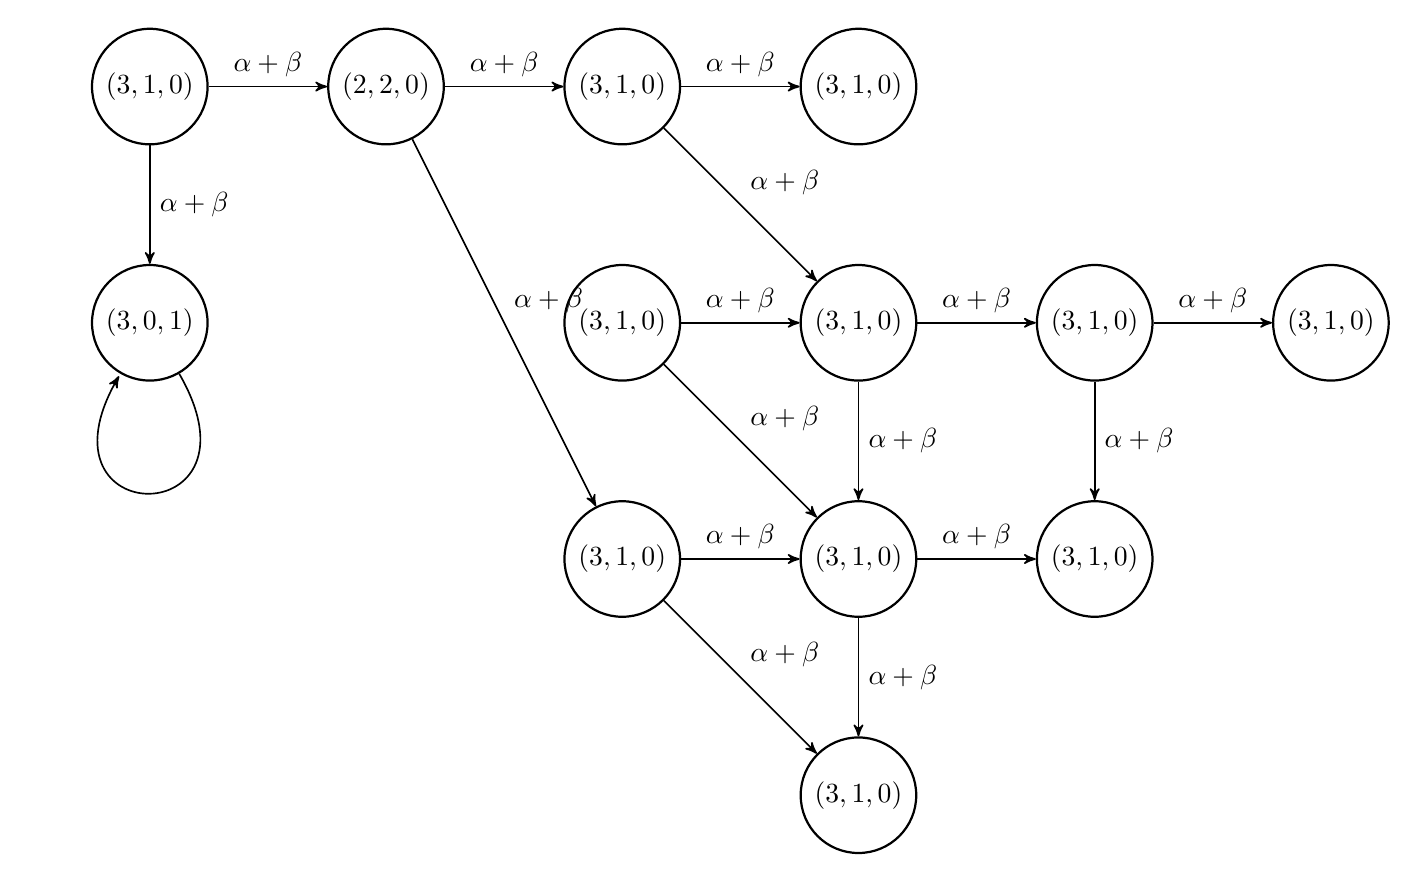
\begin{tikzpicture}[->, >=stealth', auto, semithick, node distance=3cm]
        \tikzstyle{every state}=[fill=white,draw=black,thick,text=black]
        \node[state]    (Init)                      {$(3,1,0)$};
        \node[state]    (S_301)[below of=Init]      {$(3,0,1)$};
        \node[state]    (S_220)[right of=Init]      {$(2,2,0)$};
        \node[state]    (D)[right of=S_220]         {$(3,1,0)$};
        \node[state]    (E)[below of=D]         {$(3,1,0)$};
        \node[state]    (F)[below of=E]         {$(3,1,0)$};
        \node[state]    (G)[right of=D]         {$(3,1,0)$};
        \node[state]    (H)[below of=G]         {$(3,1,0)$};
        \node[state]    (I)[below of=H]         {$(3,1,0)$};
        \node[state]    (J)[below of=I]         {$(3,1,0)$};
        \node[state]    (K)[right of=H]         {$(3,1,0)$};
        \node[state]    (L)[right of=I]         {$(3,1,0)$};
        \node[state]    (M)[right of=K]         {$(3,1,0)$};
        \path
        (Init) edge node{$\alpha + \beta$} (S_301)
            edge node{$\alpha + \beta$} (S_220)
        (S_301) edge [in=240,out=300,loop]  ()
        (S_220) edge node{$\alpha + \beta$} (D)
            edge node{$\alpha + \beta$} (F)
        (D) edge node{$\alpha + \beta$} (G)
            edge node{$\alpha + \beta$} (H)
        (E) edge node{$\alpha + \beta$} (H)
            edge node{$\alpha + \beta$} (I)
        (F) edge node{$\alpha + \beta$} (I)
            edge node{$\alpha + \beta$} (J)
        (H) edge node{$\alpha + \beta$} (K)
            edge node{$\alpha + \beta$} (I)
        (I) edge node{$\alpha + \beta$} (L)
            edge node{$\alpha + \beta$} (J)
        (K) edge node{$\alpha + \beta$} (M)
            edge node{$\alpha + \beta$} (L);
        \end{tikzpicture}
    \caption{$SIR(3,1,0)$ CTMC model with parameters$(\alpha, \beta)$}
\end{figure}

Uniformize the chain with uniformization rate $(3\alpha + 4\beta)$, we derive the following uniformized DTMC:
\begin{figure}
    \centering
    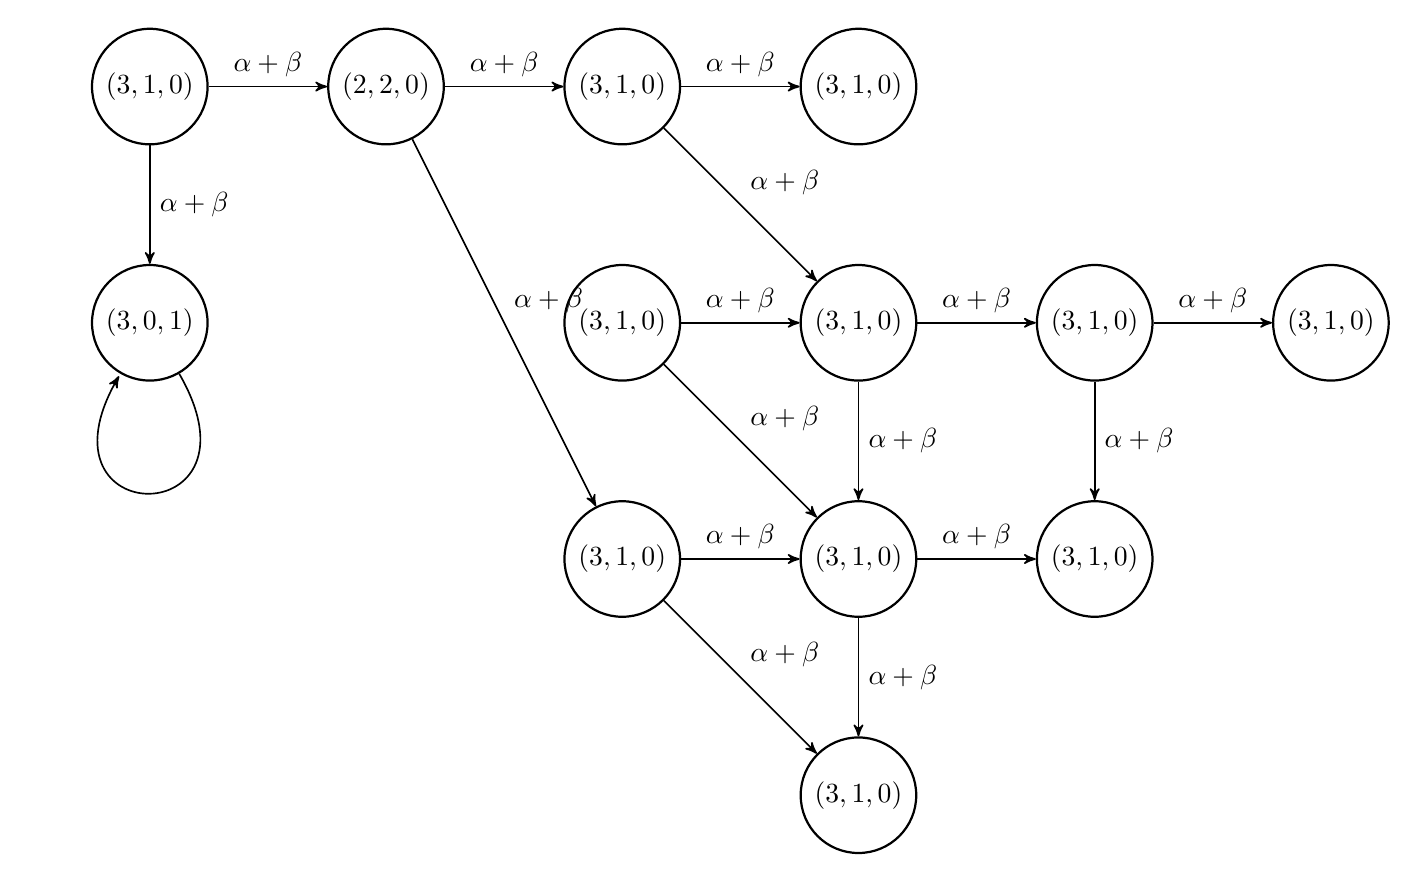
\begin{tikzpicture}[->, >=stealth', auto, semithick, node distance=3cm]
        \tikzstyle{every state}=[fill=white,draw=black,thick,text=black]
        \node[state]    (Init)                      {$(3,1,0)$};
        \node[state]    (S_301)[below of=Init]      {$(3,0,1)$};
        \node[state]    (S_220)[right of=Init]      {$(2,2,0)$};
        \node[state]    (D)[right of=S_220]         {$(3,1,0)$};
        \node[state]    (E)[below of=D]         {$(3,1,0)$};
        \node[state]    (F)[below of=E]         {$(3,1,0)$};
        \node[state]    (G)[right of=D]         {$(3,1,0)$};
        \node[state]    (H)[below of=G]         {$(3,1,0)$};
        \node[state]    (I)[below of=H]         {$(3,1,0)$};
        \node[state]    (J)[below of=I]         {$(3,1,0)$};
        \node[state]    (K)[right of=H]         {$(3,1,0)$};
        \node[state]    (L)[right of=I]         {$(3,1,0)$};
        \node[state]    (M)[right of=K]         {$(3,1,0)$};
        \path
        (Init) edge node{$\alpha + \beta$} (S_301)
            edge node{$\alpha + \beta$} (S_220)
        (S_301) edge [in=240,out=300,loop]  ()
        (S_220) edge node{$\alpha + \beta$} (D)
            edge node{$\alpha + \beta$} (F)
        (D) edge node{$\alpha + \beta$} (G)
            edge node{$\alpha + \beta$} (H)
        (E) edge node{$\alpha + \beta$} (H)
            edge node{$\alpha + \beta$} (I)
        (F) edge node{$\alpha + \beta$} (I)
            edge node{$\alpha + \beta$} (J)
        (H) edge node{$\alpha + \beta$} (K)
            edge node{$\alpha + \beta$} (I)
        (I) edge node{$\alpha + \beta$} (L)
            edge node{$\alpha + \beta$} (J)
        (K) edge node{$\alpha + \beta$} (M)
            edge node{$\alpha + \beta$} (L);
        \end{tikzpicture}
    \caption{$SIR(3,1,0)$ CTMC model with parameters$(\alpha, \beta)$}
\end{figure}
\subsection{Properties}
\subsection{Evaluation}



\chapter{Conclusion}
\section{Summary}

\begin{itemize}
    \item
\end{itemize}

\section{Future works}

\printbibliography

\end{document}